\documentclass[tikz,border=10pt]{standalone}
\usepackage{amsmath}
\usetikzlibrary{arrows.meta, calc, decorations.markings}

\begin{document}
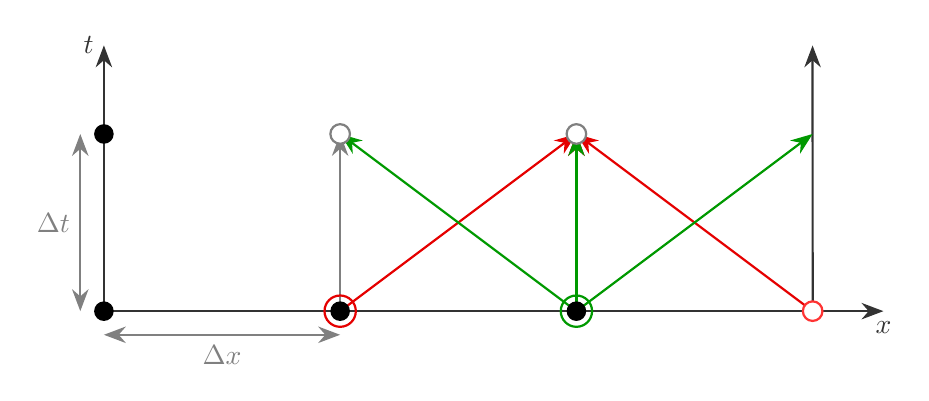
\begin{tikzpicture}[
    scale=1.5,
    >={Stealth[scale=1.2]},
    axis/.style={->, thick, black!80},
    dimline/.style={<->, thick, gray},
    dot/.style={circle, fill=black, inner sep=2.5pt, outer sep=0pt},
    hollow/.style={circle, draw=gray, thick, fill=white, inner sep=2.5pt, outer sep=0pt},
    ring/.style={circle, thick, inner sep=4pt},
    ghost/.style={circle, draw=red!80, thick, fill=white, inner sep=2.5pt}
]

    \def\dx{2.0}  
    \def\dt{1.5} 
    \def\xmax{3}  

    \foreach \x in {0,1,2,3} {
        \coordinate (B\x) at (\x*\dx, 0);
        \coordinate (T\x) at (\x*\dx, \dt);
    }

    \draw[axis] (B0) -- (0, 1.5*\dt) node[left] {$t$};
    \draw[axis] (B0) -- (3.3*\dx, 0) node[below] {$x$};
    \draw[axis] (B3) -- (3*\dx, 1.5*\dt);

    \draw[dimline] (-0.2, 0) -- (-0.2, \dt) 
        node[midway, left] {$\Delta t$};
    \draw[dimline] (0, -0.2) -- (\dx, -0.2) 
        node[midway, below] {$\Delta x$};

    \draw[->, thick, gray] (B1) -- (T1);
    \draw[->, thick, gray] (B2) -- (T2);

    \draw[->, thick, red!90!black] (B1) -- (T2);
    \draw[->, thick, red!90!black] (B3) -- (T2);

    \draw[->, thick, green!60!black] (B2) -- (T1);
    \draw[->, thick, green!60!black] (B2) -- ($(B2)!1.0!(T3)$);
    \draw[->, thick, red!90!black] (B2) -- (T2);

    \draw[->, thick, green!60!black] (B2) -- (T2);
    \node[dot] at (B0) {};
    \node[dot] at (B1) {};
    \node[ring, draw=red!90!black] at (B1) {}; 
    \node[dot] at (B2) {};
    \node[ring, draw=green!60!black] at (B2) {};
    \node[ghost] at (B3) {};
    \node[dot] at (T0) {};
    \node[hollow] at (T1) {};
    \node[hollow] at (T2) {};
    
\end{tikzpicture}
\end{document}
